\documentclass[a4paper,12pt]{article}

\usepackage[utf8]{inputenc}
\usepackage{amsmath, amssymb}
\usepackage{graphicx}
\usepackage{hyperref}
\usepackage{pdfpages}
\usepackage{enumitem}
\usepackage{array}
\usepackage{longtable}
\usepackage{comment}

\title{Pretest Practice}
\author{Niccolò Gabrielli}
\date{\today}

\newcolumntype{C}[1]{>{\centering\arraybackslash}m{#1}}  % Centered m-column






\begin{document}

\maketitle

\tableofcontents
\newpage


\section{24-01-2025}

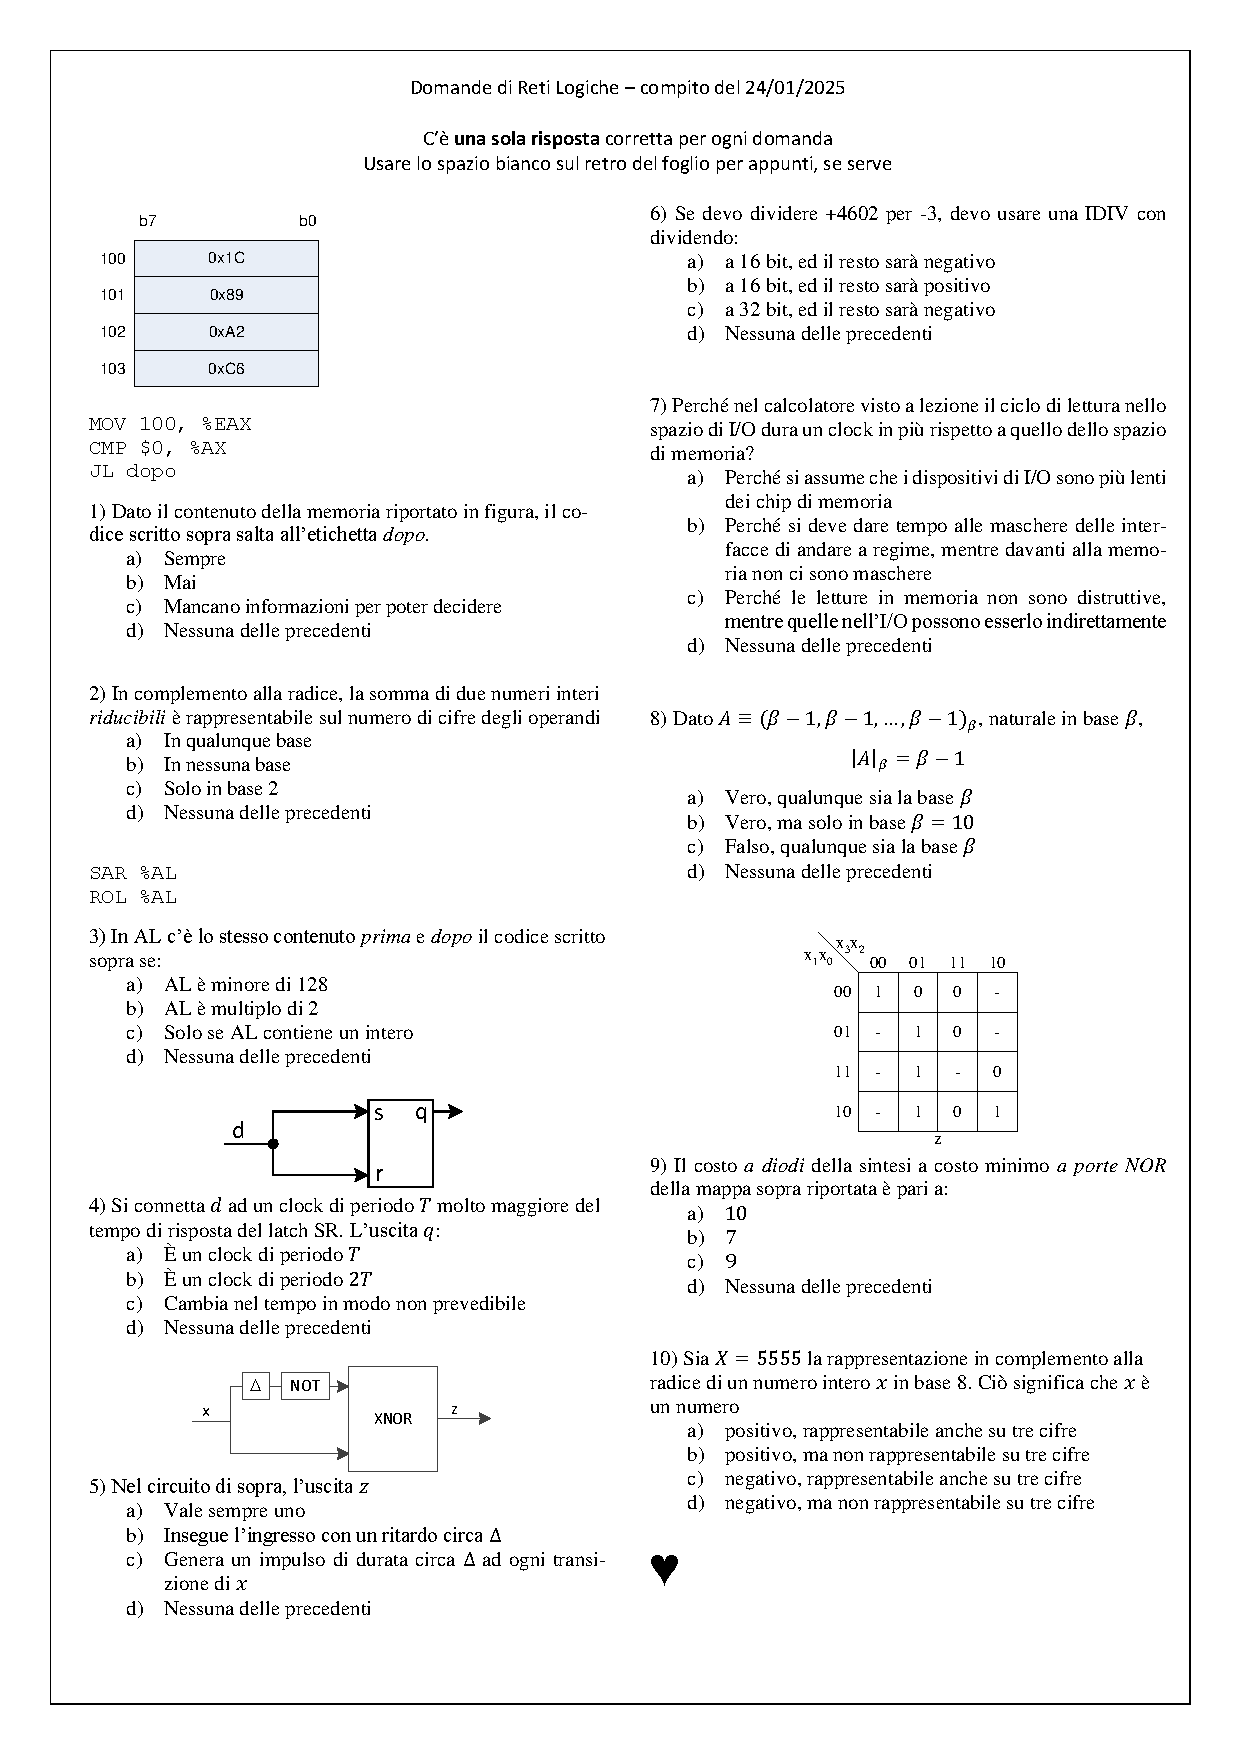
\includegraphics[width = \textwidth]{pretestImage/Domande RL 20250124.pdf}

\noindent\hspace*{-1.5cm}
    \begin{tabular}{|C{0.7cm}|C{8cm}|C{8cm}|}
        \hline
        \textbf{\#} & \textbf{High-level} & \textbf{Solution} \\
        
        \hline
        
        1 
        &
        I need to know how MOV moves data into registers $($ in what order $)$
        & 
        \begin{itemize}[label=$\rightarrow$]
            \item We're working in \textbf{little-edian} so the least significant byte is stored in the lowest address
            \item Smallest + i = smallest + i, iterated for each 9 bit memory address
        \end{itemize}   
        \\
        
        \hline


        2
        &
        Need to understand the conditions for a \textbf{riducibile} integer, and the arithmetic of riducibile numbers
        &
         \begin{itemize}[label=\(\rightarrow\)]
            \item Definition of a reducible integer in Anki 
            \item Worst case scenario is the addition between natural numbers, which works
            \item Given all the \textit{other bases} can be \textbf{represented} in base 2, if it works in base 2, it works in all 
        \end{itemize}   
        \\

        \hline

        3
        &
        Need to understand how SAR, SHR, ROL, etc. work
        &
         \begin{itemize}[label=\(\rightarrow\)]
            \item Stiamo ommettendo il sorgente quindi si fa solo 1 volta
            \item ROL takes the last bit and puts it in both CF and the first bit and shifts everything to the left
            \item \textit{Nothing is conserved} given that we're \textit{not using the CF flag} for intermediary stuff
        \end{itemize}
        
        \\

        \hline

        4
        &
        Need to know how latch SR's work    
        &
        \begin{itemize}[label=\(\rightarrow\)]
            \item Can't change variables at the same time in microprocessors $\Rightarrow$ we're going to pass through an intermediary state in which we don't know what will happen 
        \end{itemize} 
        \\

        \hline

    \end{tabular}


\noindent\hspace*{-1.5cm}
    \begin{tabular}{|C{0.7cm}|C{8cm}|C{8cm}|}
        \hline



        5
        &
        Need to know how an XNOR gate works        
        &
        \begin{itemize}[label=\(\rightarrow\)]
            \item XNOR only provides 1 if both the imputs are the same $\Rightarrow$ generatore di impulso
        \end{itemize}
        \\
        \hline        


        6
        &
        Need to understand how IDIV works
        &
        \begin{itemize}[label=\(\rightarrow\)]
            \item Relationship with dividendo and divisore bit sizes, if dividendo is 16 bits $\Rightarrow$ the divisore was 8 bits
            \item See if the quoziente is representable on 8 bits 
            \item IDIV also \textbf{does not obide} by \textbf{univoco} condition, it just does truncation
        \end{itemize}
        \\
        \hline


        7
        &
        Really learn the structure of a calculator which is really important knowledge
        &
        \begin{itemize}[label=\(\rightarrow\)]
            \item TODO
        \end{itemize}

        \\
        \hline


        8
        &
        Need to know what the notation means
        &
        \begin{itemize}[label=\(\rightarrow\)]
            \item the A $\equiv \beta-1, \beta-1, ..., \beta-1 $ means that we just have $\beta-1$ in each position
            \item Then the $|A|_{\beta} = \beta-1$ means the value I think in decimal
            \item Doing the math it comes out to be true and it'll be true in all bases
        \end{itemize}

        \\
        \hline


        9
        &
        This is elementary mappe di karnaugh stuff
        &
        \begin{itemize}[label=\(\rightarrow\)]
            \item Sintesi a porte NOR you flip then reflip, just look at the ingressi because you don't optimize those
        \end{itemize}
        \\
        \hline


        10
        &
        Problem on the riducibilità of numbers, goes back to arithmetic 
        &
        \begin{itemize}[label=\(\rightarrow\)]
            \item First see if the first cifra is $> \frac{\beta}{2}$ to see if it's negative
            \item Look at the representability of individual cifre in the reduced form
            \item Or see the condition of the represetability by still looking at the most significant bit and see if the last and penultimate bit are equal to each other
        \end{itemize}
        \\
        \hline

    \end{tabular}



\section{08-01-2025}

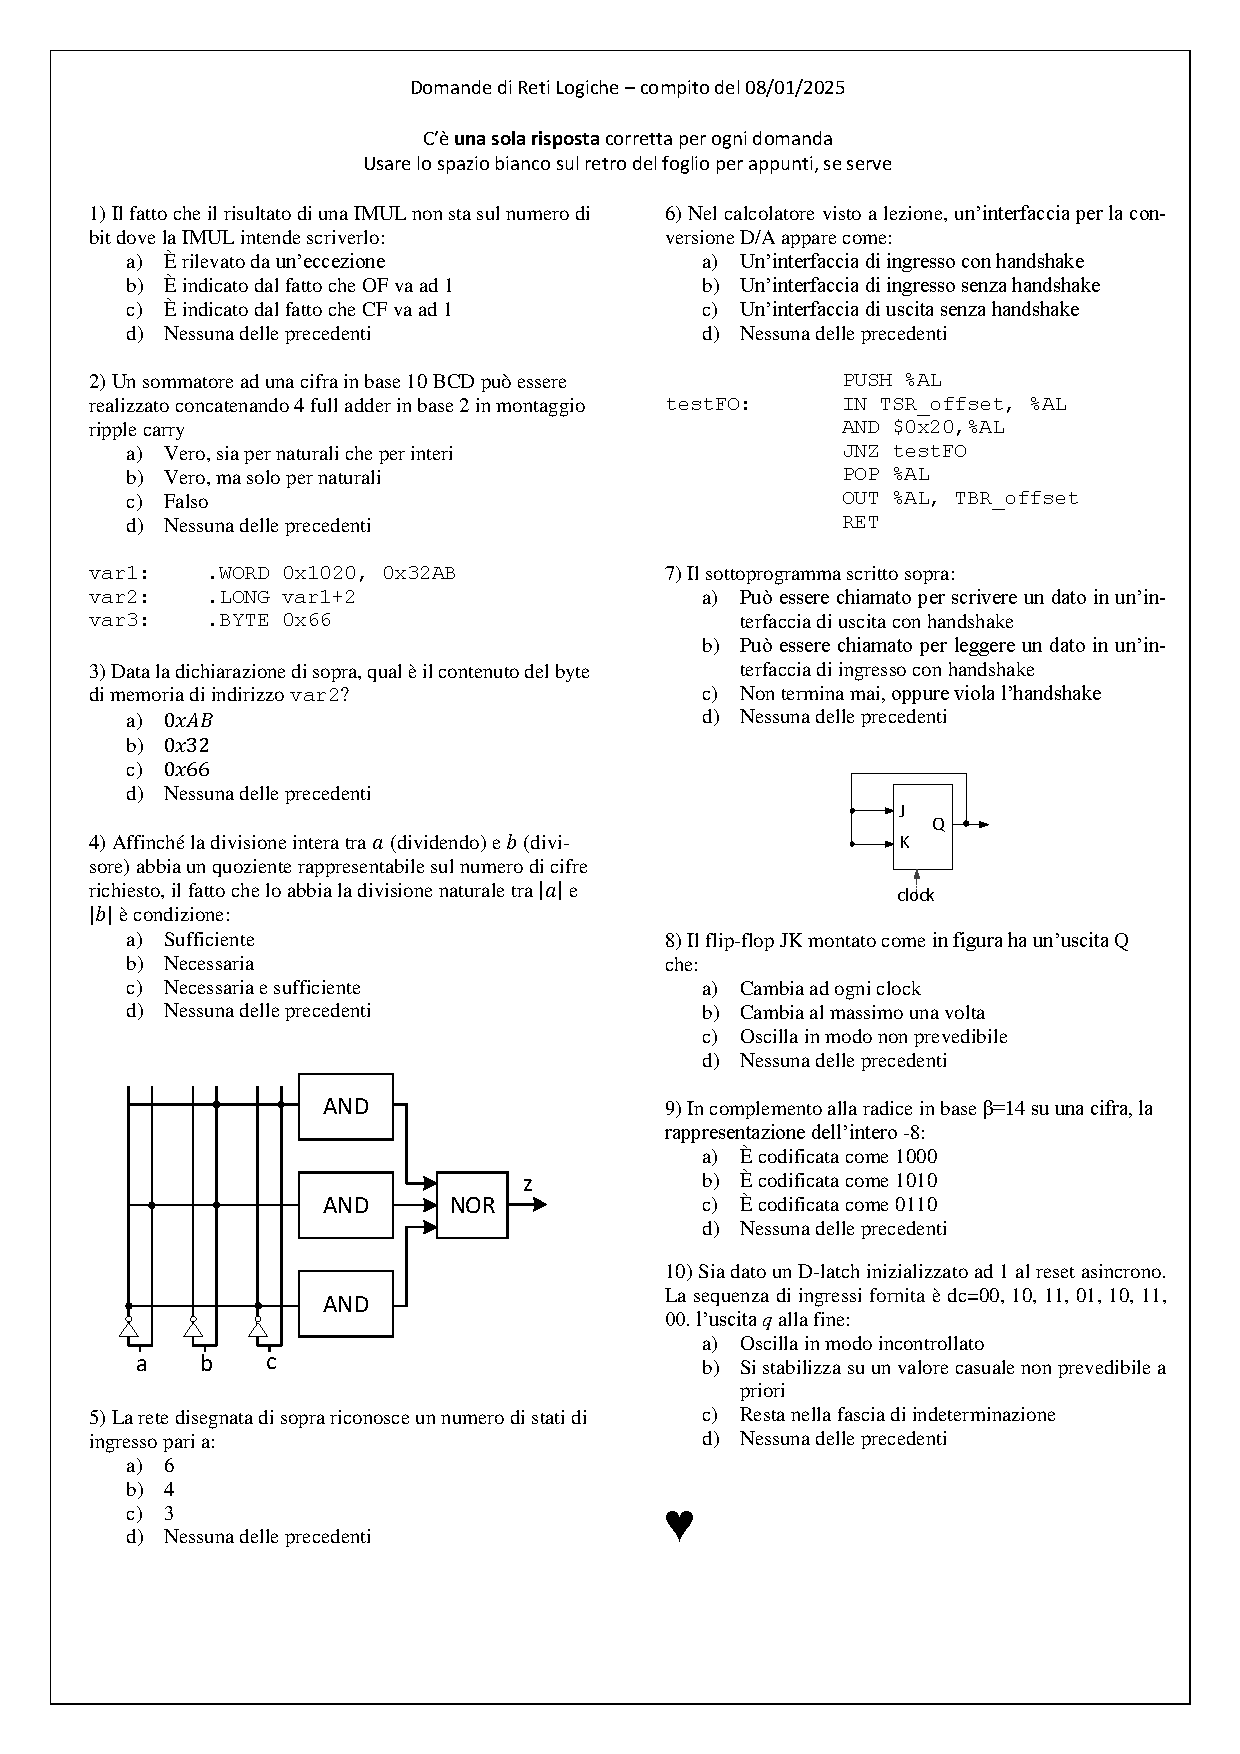
\includegraphics[width = \textwidth]{pretestImage/Domande RL 20250108.pdf}
\newpage

\noindent\hspace*{-1.5cm}
    \begin{tabular}{|C{0.7cm}|C{8cm}|C{8cm}|}
        \hline
        \textbf{\#} & \textbf{High-level} & \textbf{Solution} \\
        \hline

        1
        &
        Gotta know which flags are impacted by assembler operations
        &
        \begin{itemize}[label=\(\rightarrow\)]
            \item In IMUL \& MUL both CF e OF vengono modificati
            \item Just fyi, in IDIV \& DIV, viene generato un'interruzione interno
        \end{itemize} 
        \\

        \hline

        2
        &
        If the result needs to be in BCD, it doesn't work
        &
         \begin{itemize}[label=\(\rightarrow\)]
            \item Just using 4 full adders, i would get the correct answer in bits
            \item However, the representation of the result in BCD would require adding +6 to the answer
        \end{itemize}
        \\

        \hline

        3
        &
        Knowing what variables are in assembler.
        &
         \begin{itemize}[label=\(\rightarrow\)]
            \item Variables are just memory addresses
            \item The problem has var2 the address of the third byte pointed by var1
            \item We don't know what the address is though 
        \end{itemize}
        \\


        \hline

        4
        &
        Understanding the relationship between numeri naturali and interi. Understanding the meaning of condizione sufficiente e necessaria         
        &
         \begin{itemize}[label=\(\rightarrow\)]
            \item Divisione intera is a special case of divisione naturale from a representation standpoint
            \item $\Rightarrow$ condizione necessaria 
        \end{itemize}
        \\

        \hline

        5
        &
        Understand how gates work $\rightarrow$ write out the tabella di verità $\rightarrow$ see how many states are 'riconosciuto' $\Rightarrow$ uscita == 1
        &
         \begin{itemize}[label=\(\rightarrow\)]
            \item Following the steps above I get to 3
        \end{itemize}
        \\
        \hline

        6
        &
        Know more about the struttura del calcolatore
        &
         \begin{itemize}[label=\(\rightarrow\)]
            \item Full answer is literally written in the notes, \textit{interfaccia di uscita senza handshake}
        \end{itemize}
        \\
        \hline

    \end{tabular}


\newpage

\noindent\hspace*{-1.5cm}
    \begin{tabular}{|C{0.7cm}|C{8cm}|C{8cm}|}
        \hline
        \textbf{\#} & \textbf{High-level} & \textbf{Solution} \\
        \hline
        
        7
        &
        Need to understand how the flags work, and how the AND operation works
        &
         \begin{itemize}[label=\(\rightarrow\)]
            \item We want FO to be 1 in order to be able to write something new
            \item AND replaces in the operando destinatario the \textit{result} of and \textbf{AND} gate of each bit
            \item The important part is that we have JNZ which means that if the FO flag is 1, we stay in the loop, which isn't correct
        \end{itemize}
        \\
        \hline


        8
        &
        Need to understand how the flip flop JK works.
        &
         \begin{itemize}[label=\(\rightarrow\)]
            \item ANKI for flip-flop JK
            \item Changes at most one time based on how the flip-flop JK words
        \end{itemize}
        \\
        \hline
        

        9
        &
        Need to know how complemento alla radice works
        &
         \begin{itemize}[label=\(\rightarrow\)]
            \item -8 is out of the range of representable numbers in complemento alla radice in base $\beta$ = 14
        \end{itemize}
        \\
        \hline


        10
        &
        Need to know how a D-latch works, and an important physical detail where variables do not change simultaneously
        &
         \begin{itemize}[label=\(\rightarrow\)]
            \item The d-latch passes over 10 or 01 when going from 11->00, so we don't know the last value
        \end{itemize}
        \\
        \hline
        
    \end{tabular}



\newpage

\section{15-07-2025}



\end{document}






\begin{comment}

        &

        &
         \begin{itemize}[label=\(\rightarrow\)]
            \item 
        \end{itemize}
        \\
        \hline

\end{comment}